\documentclass[fr]{../../../../../../eplexam}
\usepackage{../../../../../../eplunits}

\hypertitle{Mécanique des milieux continus}{4}{MECA}{1901}{2017}{Août}{Mineure}
{Martin Braquet}
{Issam Doghri et Philippe Chatelain}

\section{Théorie}
\begin{enumerate}
	\item Interpréter le terme $\epsilon_{12}$ du tenseur des déformations infinitésimales.\\ Utiliser un dessin pour votre explication.
	\item Donner deux types de décomposition de tenseur et illustrer leur utilisation dans les concepts vus au cours.
	\item En bref, qu'énonce le théorème de Green-Naghdi-Rivlin? Expliquez brièvement comment le prouver.
	\item Illustrez le principe d'admissibilité (thermodynamique) dans son utilisation pour établir deux lois de comportement (Mécanique des fluides, élasticité, transfert de chaleur,\dots).
\end{enumerate}

\nosolution

\section{Plaque mince sur double appui}
Une plaque mince occupe avant déformation le domaine \( (x,y,z) \in \left[-\frac{l}{2} , \frac{l}{2}\right] \times \left[-\frac{c}{2}, \frac{c}{2}\right] \times \left[-\frac{b}{2}, \frac{b}{2}\right] \). La plaque repose sur deux appuis en \( \left(x=\pm \frac{l}{2}, y=\frac{c}{2}\right) \) et est soumise à son poids propre représenté par une force volumique en tout point $f_y = \rho g$ ($\rho$ désignant la masse volumique et $g$ l'accélération due à la pesanteur). On montre que les seules composantes non nulles du champ de contraintes sont données comme suit en coordonnées cartésiennes:\\
$$\frac{\sigma_{xx}(x,y)}{\rho g} = \left[-\frac{3}{5}+\frac{3}{2}\left(\frac{l}{c}\right)^2-6\left(\frac{x}{c}\right)^2 + 4\left(\frac{y}{c}\right)^2\right]y$$
$$\frac{\sigma_{yy}\left(x,y\right)}{\rho g} = \left[\frac{1}{2}-k\left(\frac{y}{c}\right)^2\right]y$$
$$\frac{\sigma_{xy}\left(x,y\right)}{\rho g} = \left[-\frac{3}{2}+k'\left(\frac{y}{c}\right)^2\right]x$$
où \( k \) et \( k' \) sont des constantes.
\begin{enumerate}
	\item Ecrire les conditions d'équilibre en tout point et en déduire les valeurs de \( k \) et \( k' \).
	\item Ecrire et vérifier les conditions frontières en $ y = \frac{c}{2}$ et $ y = -\frac{c}{2}$.
	\item En chacun des deux appuis \( \left(x = \pm \frac{l}{2}, y=\frac{c}{2}\right) \), il y a une force de réaction verticale égale à la moitié du poids propre total de la plaque, et un moment de réaction nul. Ecrire et vérifier les conditions frontières en $x = \pm \frac{l}{2}$  selon de Saint-Venant.
	\item Pour $l = 10c$.
        \begin{enumerate}
            \item Calculer les contraintes en $x= 0$. 
            \item Quelle est la composante la plus importante en valeur absolue?
            \item Tracer l'allure de cette composante en fonction de y.
            \item Si le matériau est fragile, indiquer l'endroit et la direction de propagation de la première fissure.
        \end{enumerate}
	\item Egalement pour $l = 10c$.
        \begin{enumerate}
         \item Calculer les contraintes en $x=\frac{l}{2}$.
         \item Quelle est la composante la plus importante en valeur absolue?
         \item Tracer l'allure de cette composante en fonction de \(y\).
        \end{enumerate}
\end{enumerate}
\begin{center}
	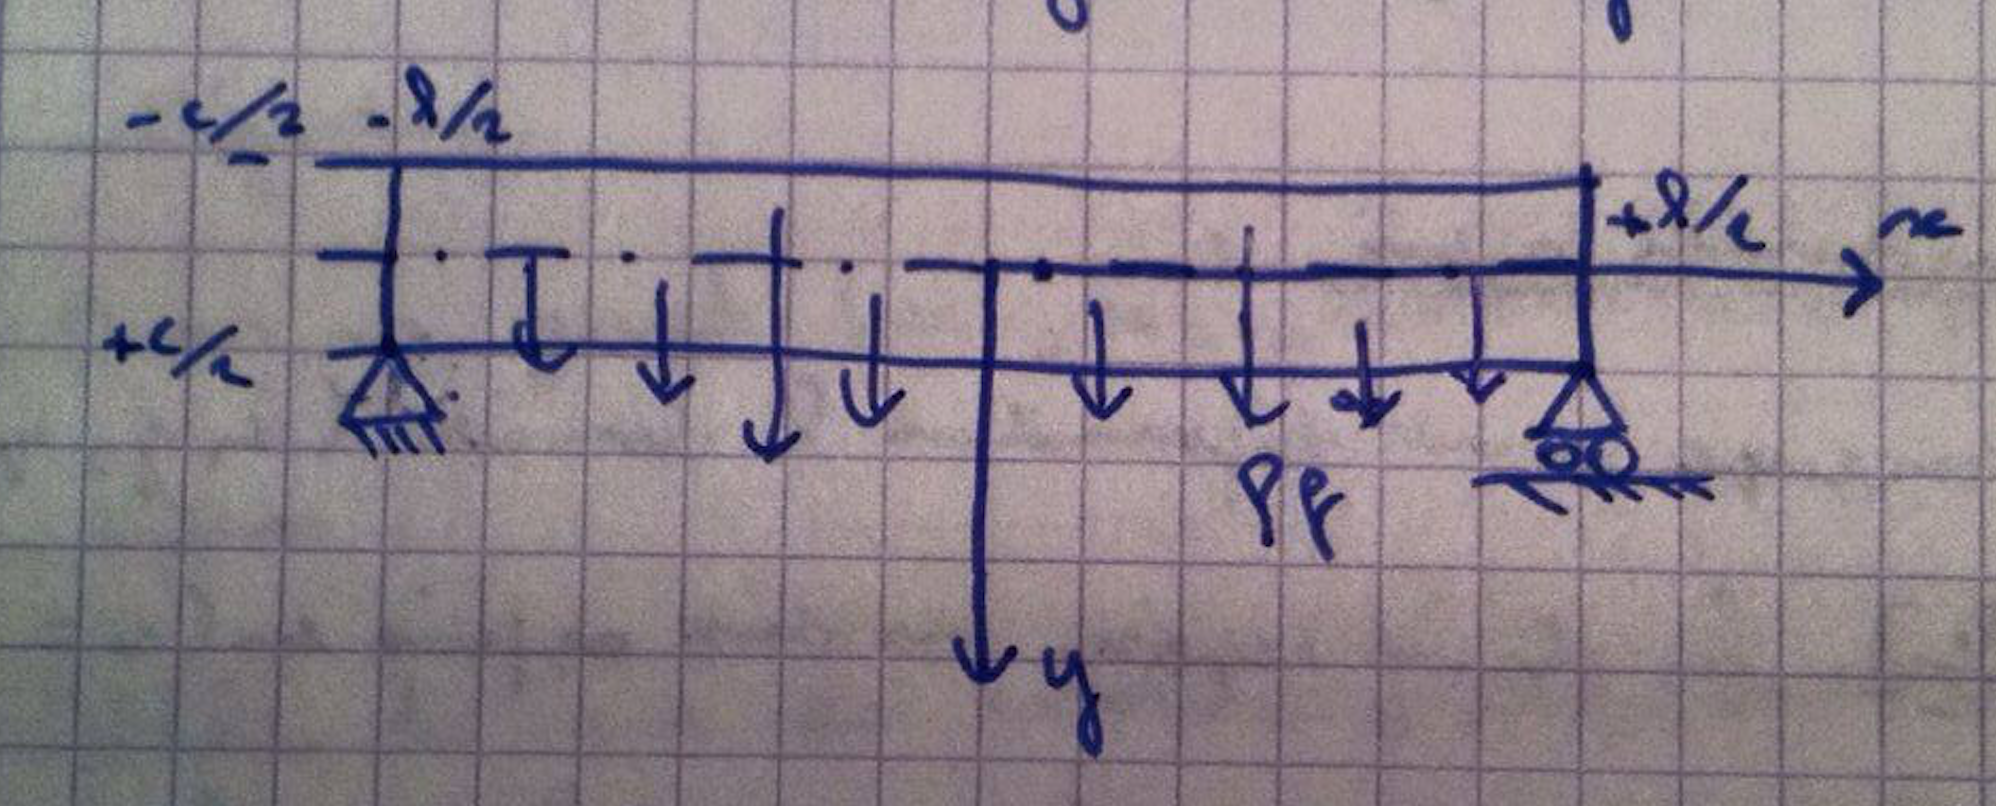
\includegraphics[scale=0.25]{I2.png}
\end{center}

\nosolution

\section{Couette entre deux plaques plânes poreuses}
On étudie l'écoulement stationnaire et incompressible d'un fluide visqueux newtonien entre 2 plaques planes poreuses. Celles-ci sont situées en $x_2 = 0$ et $x_2 = h$, et sont de longueur $L\gg h$. La plaque inférieure est fixe, tandis que la plaque supérieure se déplace parallèlement à la plaque inférieure, à la vitesse $ U (\si{m/s})$. De plus, au travers de la plaque inférieure, du fluide est injecté dans le canal. Le débit volumique par unité de surface à l'injection est uniforme et vaut $q_0 (\si{m/s})$. Sur la plaque supérieure par contre, on procède à l'extraction d'une certaine quantité de fluide. L'injection et l'extraction de fluide se produisent dans la direction normale à la paroi ( qu'elle soit fixe ou en mouvement). En d'autres mots, une composante normale de vitesse s'ajoute à celle liée au déplacement éventuel des plaques. Les plaques étant très longues, on négligera les effets se produisant aux extrémités. On considère en outre le problème comme établi. Enfin, il n'y a pas de forces de volume. Le fluide est décrit par une masse volumique $\rho$ et une viscosité dynamique de cisaillement $\mu$.
\begin{enumerate}
	\item Faire des hypothèses justifiées sur la forme des champs de vitesse et de pression dans le domaine situé entre les plaques.
	\item Quelles sont les conditions frontières pour les différentes composantes du champ de vitesse?
	\item Obtenir l'expression de la composante verticale du champs de vitesse $v_2$.
	\item Montrer que l'équation à résoudre pour obtenir la composante horizontale du champs de vitesse $v_1$, peut s'écrire sous la forme \( v_1'' - k_1 v_1'= k2 \).
	
	Donner l'expression des constantes $k_1$ et $k_2$.
	\item Résoudre l'équation obtenue ci-dessus. Déterminer la valeur des constantes d'intégration.
	\item Dans un graphe \( (v_1,x_2) \), dessiner le profil de la composante horizontale de vitesse.
	\item Calculer le taux de rotation d'un élément matériel dans le canal. Commenter son signe et son profil.
	\item Calculer la trajectoire d'une particule se trouvant en \( (x_1,x_2)  = (0,0) \) en $t = 0$.
	\item Pendant combien de temps une particule restera-t-elle entre les deux plaques?
	\item Grâce à sa définition, calculer la composante horizontale de la densité des forces de contact (i.e cisaillement) sur la plaque inférieure.
	\item Obtenir ce résultat au travers d'une analyse sur un volume de contrôle.
\end{enumerate}

\nosolution

\end{document}
